\subsection{Modèle LNAS}
Nous décrivons ici le modèle LNAS (Long Normal Allocation and Senescence) appliqué au blé. C’est un modèle innovant et suffisamment simple pour illustrer tous les enjeux de la thèse. Il est plutôt robuste étant donné sa simplicité, et le faible nombre de données et paramètres requis le rend pratique à l’utilisation. Il traite la production de biomasse au niveau compartemental et peut être considéré comme une simplification du modèle Greenlab qui décrit les même processus au niveau des organes.
C’est un modèle Markovien en temps discret.

Le modèle décrit comment la biomasse produite quotidiennement est allouée aux différents organes avec des fonctions d'allocations propres à chaque types d'organes :
\[ o = \{\mathrm{g:grain, s:tige, r:racines, g : feuilles~vertes}\} \]

La circulation de la biomasse est décrite par trois fonctions $\alpha$,$\beta$ et $\gamma$ qui représentent respectivement l'allocation de la biomasse disponible à chaque type d'organe, la remobilisation de la biomasse d'un organe dans le pool commun de biomasse et la sénescence d'un organe.

\begin{figure}[h]
\centering
  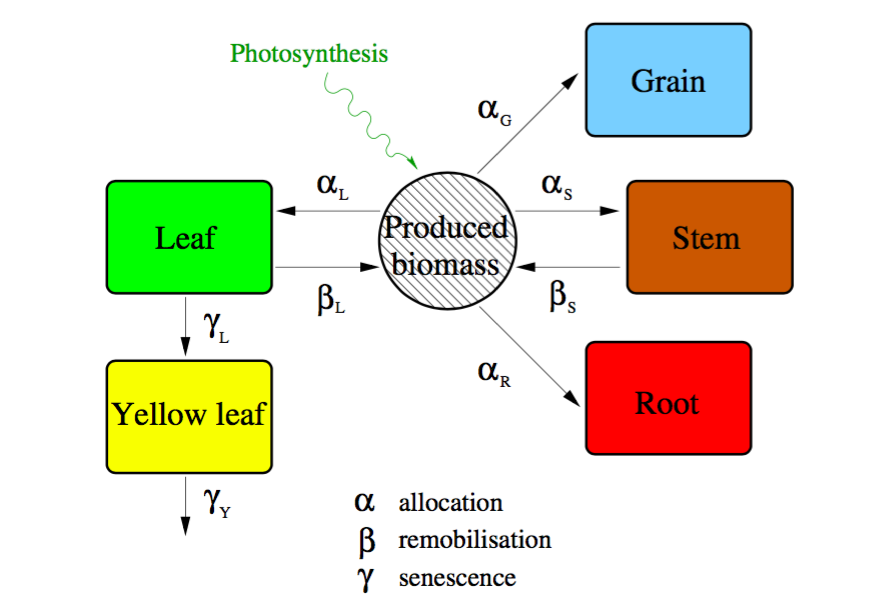
\includegraphics[scale=0.37]{./img/schema-lnas.png}
  \caption{Modélisation de la circulation de biomasse au sein de la plante (modélisée comme un ensemble de compartiments d'organes différents) par des fonctions d'allocation, de remobilisation et de sénescence.}
  \label{fig:circulation_biomasse}
\end{figure}



A chaque temps $n$, on redistribue la biomasse disponible, notée $q^{(n)}$, qui est la somme de la biomasse produite par photosynthèse et de la biomasse réallouée par les organes.

On formalise ce modèle par leurs expressions mathématiques : 
la biomasse de l'organe o, noté $Q_o$ est donnée par :
\[ {Q_o^{(n+1)}} = (1-\beta_o^{(n)}-\gamma_o^{(n)} )(Q_o)^{(n)} +\alpha_o^{(n)}q^{(n)} \]

En supposant que la répartition de biomasse ne commence qu'après un temps caractéristique $\tau_g$ nous pouvons paramétrer la fonction d'allocation $\alpha$ avec la loi log-normale :
\[ {\alpha_g^{(n)}}=F_{\log N(\mu_s,\sigma_g)}(\tau^{(n)}-\tau_g)=\frac{1}{2} (1+\erf[\frac{1}{\sigma_g \sqrt{2}}\log\left(\frac{\tau^{(n)}-\tau_g}{t_{1/2}-\tau_g}\right) \]

Les autres fonctions d'allocations $\beta$ et $\gamma$   peuvent se déduire de l'expression de $\alpha_g^{(n)}$.
Ces trois fonctions $\alpha$, $\beta$ et $\gamma$ sont paramétrées par rapport au temps thermique qui peut s'écrire :

\[ {\tau}^{(n+1)}=\tau^{(n)}+\max[0,\underline{T}^{(n)}-Tc] \]

La quantité de biomasse disponible au jour n est donnée par l'expression de $q^{(n)}$ :
\[ 
{q^{(n)}} = \text{RUE}\cdot \min[SSI^{(n)}, TSI_\uparrow^{(n)}]\underline{PAR}^{(n)}(1-e^{-\lambda LAI^{(n)}})+\sum_o \beta_o^{(n)}Q_o^{(n)} 
\]
Nous nous baserons sur un document fourni par le client lors de l'implémentation de ce modèle, ce document contenant les formules mathématiques nécessaires.

